\chapter{Asking Miami Moguls How They Got Rich!}

There is no blackboard in this lecture, but there is an argument. We are taken first through spectacle and then through a sequence of mechanisms: search, access, recognition, sales psychology, service systems, startup budgets, asset allocation, debt coverage, and finally the threshold at which income from assets begins to carry a life. The right way to read the lecture is not as a pile of millionaire quotes, but as a progressively sharper inquiry into how wealth becomes structurally durable.

\section{From Spectacle to Search}

The lecture opens in the mode of interruption. A stranger is stopped on the street. A Rolls Royce appears. A restaurant owner reports extraordinary revenue. A nine-figure entrepreneur speaks as if risk were almost beneath discussion. This opening does important work, but it is not yet the true beginning. The true beginning comes with the rewind: the host tells us that it is early in the morning, that he is flying from Austin to Miami, and that the point of the trip is to find some of the wealthiest people in the city and ask how they got there.

So the lecture quickly shifts from display to method. Miami is introduced as a place where wealth has thickened visibly, and that claim is given a numerical edge by the statement that the city now has \(75\%\) more millionaires than it did a decade ago. We may write the host's framing claim compactly as
\begin{equation}
M_{\mathrm{Miami,now}} \approx 1.75\,M_{\mathrm{Miami,10y}},
\end{equation}
where \(M_{\mathrm{Miami,10y}}\) and \(M_{\mathrm{Miami,now}}\) denote, respectively, the millionaire counts a decade ago and now. This is not a derived law of urban wealth; it is the lecture's opening condition. It tells us why Miami is being treated not merely as scenery, but as an experimental field.

The more interesting point is methodological. The host is not trying simply to collect glamorous stories. He wants to find what is hidden beneath visible luxury: what business structure, what operating rule, what investment habit, what discipline of risk or restraint. That is the question that governs everything that follows.

\section{Design District: Access Before Theory}

The first stop is the Design District, and the lecture refuses to pretend that this inquiry will proceed smoothly. There are refusals. There are brush-offs. There is one encounter in which recognition almost turns into cooperation and then is pulled back. There is another in which a likely subject is a fan of the channel but too busy, even on a Saturday, to stop for more than a minute. These are not dead moments. They show that access is itself one of the lecture's themes. Wealth does not simply volunteer itself for analysis; one has to track it, catch it, and sometimes miss it.

This matters because the first strong interview, with Johnny, arrives only after a visible process of filtering. The lecture thereby earns its first large claims.

Johnny reports numbers that are impossible to ignore. He gives a year above one hundred million dollars, speaks of a career total above two billion dollars, and later places annual business in the range of one hundred fifty to one hundred seventy million dollars:
\begin{align}
R_{\mathrm{Johnny},2021} &> \$100\,\mathrm{M},\\
R_{\mathrm{Johnny,annual}} &\in [\$150\,\mathrm{M},\,\$170\,\mathrm{M}],\\
S_{\mathrm{Johnny,career}} &> \$2\,\mathrm{B}.
\end{align}
These are self-reported figures, and the lecture never asks us to treat them as audited accounts. Their force is local: they justify the seriousness of the exchange.

The first principle he offers is psychology. Understand human nature. Do not push people. This comes before any formal account of capital or systems, and that ordering is important. In the lecture's rhythm, money begins in perception and in the ability to read another person. Only after that do we hear about scale, risk tolerance, or access to bank money.

A second principle is self-funding. Johnny insists that he did it himself and that only later did banks begin to seek him out. The lecture does not build a full capital-stack analysis here, but the causal sequence is clear enough: first one proves the vehicle, then the financial world becomes interested in helping it expand.

A third principle is personal liquidity. When asked for the best financial advice he ever received from a mentor, his answer is brief and striking: take the money; do not keep putting it all back in. We should not force a formal theorem where the lecture has given us a maxim. But we can already feel the distinction that will later become much sharper with Anthony Powell: there is active income, and there is the question of what one does with it once it has been earned.

\subsection{Question \& Answer: What Do We Do About a Bad Month?}

This is the first real local tension in the lecture, and it is posed exactly where it ought to be posed. The numbers are large, the tone is bold, the business history sounds invulnerable; therefore the obvious question is what happens when conditions turn against you.

Johnny's answer is almost perversely simple. He says he could never understand the idea of a bad month, and that after a certain point in his career he had not had one. We should not turn this into a universal model of business cycles. The point is not that downturns do not exist. The point is that the lecture is showing us a particular entrepreneurial temperament: one in which opportunity is seized so aggressively, and scale is reached so forcefully, that the speaker no longer narrates his business life in the language of fragile monthly survival.

He later supplies the lecture's aphoristic compression of this outlook:
\begin{equation}
\text{opportunity} + \text{preparation} \longrightarrow \text{luck}.
\end{equation}
This is not an identity in the mathematical sense, but it does function as a rule of interpretation. Luck is not magic. Luck is what the speaker calls the event in which readiness finds its opening.

The host ends the segment with an explicit recap, calling it one of the wildest interactions on the channel. That recap is not decorative. It gives us permission to reset. We have seen wealth in its most performative register. The lecture is now ready to ask whether there are calmer and more operational versions of the same story.

\section{Poppy Steak: Service, Partners, and the Refusal of Rest}

After another failed attempt and then another chase, the lecture catches a second major figure, now attached to a Rolls Royce and to Poppy Steak. The transition matters. We move from Johnny's volatility into a more conventional business domain: hospitality.

The numbers remain large, but the tone changes. The owner says only that the business has made ``a lot,'' that the COVID years were strong, and that the enterprise keeps going up. The lecture deliberately refuses exact accounting here. Instead it extracts principles: best service, best hospitality, best team, a lot of love, and a lot of hard work. Then, when the questions move to networking and capital, the language becomes even more conservative: be honest with friends, be honest with investors, stay true and loyal to partners.

This is a useful correction to the previous segment. Wealth is not being reduced to a single entrepreneurial personality type. The lecture is showing that the underlying mechanisms may vary even when the visible markers of success are similar.

\subsection{Question \& Answer: Is There a Final State Called Financial Freedom?}

The host naturally asks for a turning point: what made the speaker stand out, what produced financial freedom, what changed the game? The answer is instructive precisely because it refuses the shape of the question. There is, he says, no final arrival. One always has to work harder. One always has to strive for more. The lecture therefore refuses to let the phrase ``financial freedom'' settle too early into a single meaning.

\begin{remark}
Later in the lecture, Anthony Powell and Eric Spofford will speak as if financial freedom is a threshold condition, something like a point at which asset income covers lifestyle. Here, by contrast, the phrase is resisted. The chapter must keep both uses in view.
\end{remark}

The section therefore plays a precise role in the whole arc. It counters flamboyant wealth talk with operational discipline and counters the fantasy of a single breakthrough with the harder idea that work, service, and partner trust may not terminate in any final rest.

\section{Self-Belief and the Gym-Business Failure Model}

The next substantial interview enters through recognition again, but now with a more autobiographical energy. The speaker sells gym equipment around the world. He has been in business for eighteen years. The lecture first lets him establish the emotional ground of his career: immigrant family background, repeated rejection, a burning desire from youth, literal scarcity, peanut-butter-and-jelly years, electric bills paid in cash, and relentless self-promotion. One especially concrete detail is the claim that he once ran four hundred Craigslist ads a week. The structure of this first half is familiar: belief precedes scale.

But the lecture does not stop there. It pivots, and when it pivots it becomes one of the most analytically precise passages in the whole chapter. The host asks why so many businesses fail. The speaker replies with a specific diagnosis from the gym world: many ventures are effectively dead before they open.

The lecture gives us the central quantities:
\begin{align}
B_{0,\mathrm{gym}} &\approx \$500{,}000,\\
E_{\mathrm{gym}} &\in [\$300{,}000,\$500{,}000],\\
L_{m,\mathrm{gym}} &= \$38{,}000/\mathrm{month}.
\end{align}
Here \(B_{0,\mathrm{gym}}\) is the notional startup budget, \(E_{\mathrm{gym}}\) the equipment spend, and \(L_{m,\mathrm{gym}}\) the monthly lease burden. What makes the passage mathematically useful is not that it gives a complete model, but that it gives enough numbers to see the scale mismatch.

\subsection{Question \& Answer: Why Do Businesses Die Before They Open?}

The lecture's answer has a clear internal order.

\begin{enumerate}
\item The founder begins with what sounds like a large budget, about half a million dollars.
\item A substantial fraction of that budget is immediately absorbed by equipment.
\item The chosen location carries a very heavy monthly rent.
\item No adequate reserve is left for payroll, carrying costs, or operating uncertainty.
\item The business therefore enters life already structurally compressed.
\end{enumerate}

A useful comparison is the annualized scale of the rent burden:
\begin{equation}
12L_{m,\mathrm{gym}} = 12 \times \$38{,}000 = \$456{,}000.
\end{equation}
This is not an upfront payment schedule. The lecture does not say that one prepays twelve months. The point is comparative. The fixed lease burden, when annualized, is already of the same order as the entire startup budget.

If we add that annualized scale to the quoted equipment range, we obtain a simple measure of how quickly the structure can outrun the initial capital:
\begin{equation}
E_{\mathrm{gym}} + 12L_{m,\mathrm{gym}} \in [\$756{,}000,\$956{,}000].
\end{equation}
Again, this is not a launch cash requirement; it is a scale comparison. But it is exactly the comparison the lecture wants us to see. The venture has taken on a structure whose first-year cost intensity can easily exceed the capital base from which it begins. That is why the speaker says many businesses fail before they even get open.

The result is that the lecture turns a motivational story into something much sharper: a budget critique. Belief matters, but belief does not repeal fixed obligations.

\section{Side Hustles, Systems, and Anthony Powell's Money Sequence}

At this point the lecture pauses and steps outside the interview rhythm. The host says that one of the greatest things he has learned running the channel is that many millionaires have some kind of side hustle. The number he gives is
\begin{equation}
p(\text{side hustle}\mid \text{millionaire}) \approx 0.45.
\end{equation}
We should keep this in its proper status. It is a host-stated statistic, not a theorem derived inside the lecture. Still, it serves an important structural purpose: it shifts the chapter from isolated stories toward income architecture.

That shift prepares the entrance of Anthony Powell, the speaker who gives the lecture its cleanest money sequence.

Anthony first speaks in the language of system. McDonald's is successful, he says, because it has a systematic approach, so systematic in fact that a teenager can run the business. He claims to have built an analogous system in direct sales, contact management, lead distribution, and digital products. The emphasis is on repeatability. The system is not a metaphor; it is the condition under which success ceases to be accidental.

Then the lecture turns from business systems to monetary systems, and the sequence is explicit.

\paragraph{Step 1.} Find a vehicle that produces substantial earned income.

\paragraph{Step 2.} Do not spend the earned income.

\paragraph{Step 3.} Invest it in assets.

To keep the lecture's structure visible on the page, we may formalize the sequence lightly. Let \(Y_{e,t}\) denote earned income, \(C_t\) consumption, \(S_t\) investable surplus, and \(A_t\) the asset base. Then
\begin{align}
S_t &= Y_{e,t} - C_t,\\
A_{t+1} &= A_t + S_t.
\end{align}
This is not Anthony's notation. It is our clean reconstruction of his spoken rule: earn, refrain from consuming all of it, then convert the remainder into assets.

\subsection{Question \& Answer: What Do We Do With the First \$10{,}000 or \$20{,}000?}

Anthony asks the natural objection himself. Everybody says ``buy assets,'' but where does one begin in practice?

His first answer is an S\&P ETF. The lecture gives a concrete example. If the market is up \(17\%\) and one has \$100{,}000 invested, then
\begin{align}
\Delta V &= rV_0,\\
\Delta V &= 0.17 \times \$100{,}000 = \$17{,}000,\\
V_1 &= V_0 + \Delta V = \$117{,}000.
\end{align}
This is deliberately elementary. The lecture is not doing finance theory here. It is doing something more practical: it is showing that money placed into an asset can move without requiring an equal increment of labor at the same instant.

He then adds the repeated-deposit rule. One contributes what one can---\$250, \$500, \$1{,}000 a month---and keeps compounding while continuing to work aggressively in the active-income vehicle. The lecture's point is not that an ETF solves everything. The point is that the conversion from labor income to asset position must begin somewhere and must be repeated.

\subsection{Question \& Answer: How Can an 8-Plex Pay the Debt Load?}

Anthony's second worked example is stronger because it makes the cash-flow structure visible. When he was broke, he says, he needed rent paid. So he bought an 8-plex. The bank lends because the property is not a personal residence in the usual sense; it is an income-producing object. The question is therefore whether the rent roll can carry the debt.

We formalize the lecture's spoken logic cautiously. Let
\begin{equation}
n=8,\qquad n_{\mathrm{paying}}=7,
\end{equation}
where one unit is treated as the owner's effective unit and seven are treated as rent-paying units. Let \(c_u\) denote the average monthly net contribution of one paying unit toward debt service, and let \(D_m\) denote the monthly debt load. Then the lecture's condition is
\begin{equation}
7c_u \ge D_m.
\end{equation}

This inequality is thin, and we should say so. It abstracts from vacancy, repairs, taxes, insurance, management, and financing detail. But it captures exactly the shape of the spoken example: seven other people pay the debt load, and the owner's position is thereby carried by the property.

\begin{figure}[h]
\centering
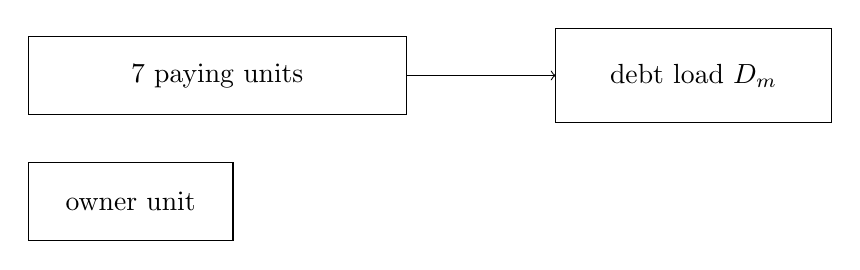
\begin{tikzpicture}[x=1cm,y=1cm]
\draw (0,0) rectangle (4.8,1);
\node at (2.4,0.5) {7 paying units};

\draw (0,-1.6) rectangle (2.6,-0.6);
\node at (1.3,-1.1) {owner unit};

\draw[->] (4.8,0.5) -- (6.7,0.5);
\draw (6.7,-0.1) rectangle (10.2,1.1);
\node at (8.45,0.5) {debt load \(D_m\)};
\end{tikzpicture}
\caption{Transcript-derived schematic of Anthony Powell's 8-plex argument. The seven paying units are said to carry the monthly debt load, leaving the owner's position effectively paid for by property cash flow.}
\end{figure}

Once the debt is carried, the lecture adds the next step: improve the property, raise its value, sell, and double the money. No full pro forma is given, so we do not invent one. What matters is the sequence:
\begin{equation}
\text{earned income} \longrightarrow \text{asset purchase} \longrightarrow \text{cash flow} \longrightarrow \text{value increase} \longrightarrow \text{liquidity event}.
\end{equation}

Anthony ends with a statement that should be heard as a class-changing rule rather than as a slogan: he does not spend earned income. The lecture wants us to understand that work may create wealth, but only assets can carry wealth forward without requiring the same labor all over again.

\section{Eric Spofford: Section 8, Cash Flow, and the Threshold of Freedom}

The final major interview takes place on a yacht, but the important movement is downward rather than upward. Eric Spofford begins with a dramatic credential---a year above one hundred million dollars and a sale of his business for \$115 million, four days before Christmas in 2021---yet the lecture uses that credential to move toward a surprisingly accessible thesis.

His business, we are told, was addiction treatment in New England, and his personal history includes addiction, recovery, and the conversion of that experience into a niche enterprise. Thus the lecture joins money to biography once again: the vehicle matters, but so does the life that discovered it.

Then comes the financial recommendation. Eric says: get into Section~8 real estate. The surrounding transcript is partly garbled, so we proceed cautiously. But the central claims are clear enough. He says the average price per property in this asset class is below \$100{,}000, that ordinary Americans can enter it, and that it produces strong cash-on-cash returns because the government overpays rent in order to incentivize the supply of low-income housing.

We may preserve the entry-price claim as
\begin{equation}
P_{\mathrm{Section8,avg}} < \$100{,}000.
\end{equation}
Again, this is the speaker's claim, not an external market survey.

The lecture then reaches its cleanest threshold statement.

\begin{definition}
In the Anthony--Eric sense of this lecture, financial freedom is reached when passive income from assets covers the recurring cost of one's life:
\begin{equation}
I_p \ge C_l.
\end{equation}
Here \(I_p\) denotes passive asset income and \(C_l\) the lifestyle cost one wishes to sustain.
\end{definition}

This is the most compressed mathematical statement in the whole chapter. It tells us why the previous sections mattered. Sales psychology, hospitality, partner honesty, startup discipline, saved earnings, ETFs, multifamily properties: all of it is being pushed toward a threshold.

\subsection{Question \& Answer: How Can an Ordinary American Become Financially Free?}

Eric answers this in an order that is easy to miss if we read too quickly.

\begin{enumerate}
\item Stop treating earned income as something to be spent immediately on lifestyle.
\item Reduce lifestyle enough to generate savings.
\item Place savings into appreciating, cash-flowing assets.
\item Repeat until the income from those assets can cover the desired life.
\item At that point the structure of action changes: one does things because one wants to, not because one must.
\end{enumerate}

This is a threshold argument rather than a luxury argument. The yacht is in the frame, but the real object is the inequality \(I_p \ge C_l\). That is the lecture's end point in mathematical form.

Eric then adds the last compression. Drugs and alcohol, he says, are for losers. One's circle matters. Loyalty should be directed toward one's future. We need not convert these claims into mathematics. Their role is different. They restore the human conditions under which the financial sequence can hold. The lecture ends, then, not only with a balance-sheet condition, but with a social and moral one: do not let your environment sabotage the structure you are trying to build.

\section{Summary}

The chapter begins with luxury as bait and ends with structure as explanation. Miami is introduced as a place where wealth is concentrated enough to be hunted. The hunt then yields several distinct mechanisms. Johnny gives us psychology, risk, self-funding, and the insistence on taking money off the table. The Poppy Steak owner gives us service, team quality, honesty, and a refusal to romanticize any final state called financial freedom. The gym entrepreneur turns scarcity into a budget model and shows how fixed costs can kill a business before it opens. Anthony Powell provides the clearest capital-allocation sequence in the lecture: earn, save, invest, let assets carry the next stage. Eric Spofford then gives us the threshold version of freedom itself.

The mathematics is sparse but decisive. We have a city-level growth claim,
\[
M_{\mathrm{Miami,now}} \approx 1.75\,M_{\mathrm{Miami,10y}},
\]
a return calculation,
\[
\Delta V = rV_0,
\]
a debt-coverage condition,
\[
7c_u \ge D_m,
\]
and finally the threshold at which work ceases to be sheer necessity,
\[
I_p \ge C_l.
\]

What the lecture finally teaches is simple to say and difficult to live. Wealth becomes durable not when it is seen, but when the structure beneath it begins to pay for itself.